%%%%%%%%%%%%%%%%%%%%%%%%%%%%%%%%%%%%%%%%%%%%%%%%%%%%%%%%%%%%%%%%%%%%
%%%%%%%%%%%%%%%%%%%%%%%%%%%%%%%%%%%%%%%%%%%%%%%%%%%%%%%%%%%%%%%%%%%%
%%                                                                %%
%% Esimerkki opinnäytteen tekemisestä LaTeX:lla 20130926          %%
%% Alkuperäinen versio Luis Costa,  muutokset Perttu Puska        %%
%%                                                                %%
%% Tähän esimerkkiin kuuluu tiedostot                             %%
%%               opinnaytepohja.tex (versio 1.7)                  %%
%%               aaltothesis.sty (versio 1.7)                     %%
%%               kuva1.eps                                        %%
%%               kuva2.eps                                        %%
%%                                                                %%
%%                                                                %%
%% Kääntäminen                                                    %%
%% latex:                                                         %%
%%             $ latex opinnaytepohja                             %%
%%             $ latex opinnaytepohja                             %%
%%                                                                %%
%%   Tuloksena on tiedosto opinnayte.dvi, joka                    %%
%%   muutetaan ps-muotoon seuraavasti                             %%
%%                                                                %%
%%             $ dvips opinnaytepohja -o                          %%
%%                                                                %%
%% Selittävät kommentit on tässä esimerkissä varustettu           %%
%% %%-merkeillä ja muutokset, joita käyttäjä voi tehdä,           %%
%% on varustettu %-merkeillä                                      %%
%%                                                                %%
%%%%%%%%%%%%%%%%%%%%%%%%%%%%%%%%%%%%%%%%%%%%%%%%%%%%%%%%%%%%%%%%%%%%
%%%%%%%%%%%%%%%%%%%%%%%%%%%%%%%%%%%%%%%%%%%%%%%%%%%%%%%%%%%%%%%%%%%%

%% Käytä toinen näistä, jos kirjoitat suomeksi:
%% ensimmäinen, jos käytät pdflatexia (kuvat on oltava pdf-tiedostoina)
%% toinen, jos haluat tuottaa ps-tiedostoa (käytä eps-formaattia kuville).
%%
%% Use one of these you write in Finnish:
%% the 1st when using pdflatex (use pdf figures) or
%% the 2nd when producing a ps file (use eps figures).
\documentclass[finnish,12pt,a4paper,pdftex]{article}
%\documentclass[finnish,12pt,a4paper,dvips]{article}





%% Käytä näitä, jos kirjoitat englanniksi
%%
%% Uncomment one of these if you write in English
%\documentclass[english,12pt,a4paper,pdftex]{article}
%\documentclass[english,12pt,a4paper,dvips]{article}

%% Tämä paketti on pakollinen
%% Valitse korkeakoulusi näistä: arts, biz, chem, elec, eng, sci.
%% Valiste editorisi käyttämä merkkikoodaustapa: utf8, latin1
%%
%% This package is required
%% Choose your school from arts, biz, chem, elec, eng, sci.
%% Choose the character encoding scheme used by your editor: utf8, latin1
\usepackage[elec,utf8]{aaltothesis} % 
%\usepackage[elec,latin1]{aaltothesis}

%% Jos käytät latex-komentoa käännettäessä (oletusarvo), 
%% kuvat kannattaa tehdä eps-muotoon. Älä käytä ps-muotoisia kuvia!
%% Käytä seuraavaa latex-komennon ja eps-kuvien kanssa 
%%
%% Jos taas käytät pdflatex-komentoa, joka kääntää tekstin suoraan
%% pdf-tiedostoksi, kuvasi on oltava jpg-formaatissa tai pdf-formaatissa.
%%
%% Use this if you run pdflatex and use jpg/pdf-format pictures.
%%
\usepackage{graphicx}
\usepackage{float}
\usepackage{gensymb}
\usepackage[%
  backend=bibtex      % biber or bibtex
% ,style=authoryear    % Alphabeticalsch
 ,style=numeric-comp  % numerical-compressed
 ,sorting=none        % no sorting
 ,sortcites=true      % some other example options ...
 ,block=none
 ,indexing=false
 ,citereset=none
 ,isbn=true
 ,url=true
 ,doi=true            % prints doi
 ,natbib=false         % if you need natbib functions
]{biblatex}
\addbibresource{viitteet.bib}  % better than \bibliography
%\bibliography{viitteet}

%% Jos et jostain syystä pidä, miten alla oleva hyperref-paketti käyttää
%% fontteja, värejä yms., käytä tämän paketin makroja muuttamaan
%% fonttimäärittelyt. Katso paketin dokumentaatiota. Paketti määrittelee
%% \url-makron, joten ota paketti käyttöön, jos et käytä hyperref-pakettia.
%%
%% Use the macros in this package to change how the hyperref package below 
%% typesets its hypertext -- hyperlink colour, font, etc. See the package
%% documentation. It also defines the \url macro, so use the package when 
%% not using the hyperref package.
%\usepackage{url}

%% Saat pdf-tiedoston viittaukset ja linkit kuntoon seuraavalla paketilla.
%% Paketti toimii erityisen hyvin pdflatexin kanssa. 
%%
%% Use this if you want to get links and nice output with pdflatex
\usepackage[pdfpagemode=None,colorlinks=true,urlcolor=red,%
linkcolor=blue,citecolor=black,pdfstartview=FitH]{hyperref}

%% Matematiikan fontteja, symboleja ja muotoiluja lisää, näitä tarvitaan usein 
%%
%% Use this if you write hard core mathematics, these are usually needed
\usepackage{amsfonts,amssymb,amsbsy}  


%% Vaakasuunnan mitat, ÄLÄ KOSKE!
\setlength{\hoffset}{-1in}
\setlength{\oddsidemargin}{35mm}
\setlength{\evensidemargin}{25mm}
\setlength{\textwidth}{15cm}
%% Pystysuunnan mitat, ÄLÄ KOSKE!
\setlength{\voffset}{-1in}
\setlength{\headsep}{7mm}
\setlength{\headheight}{1em}
\setlength{\topmargin}{25mm-\headheight-\headsep}
\setlength{\textheight}{23cm}

\usepackage{setspace}  % KYPSYYSNÄYTETTÄ VARTEN


%% Kaikki mikä paperille tulostuu, on tämän jälkeen
%%
%% Output starts here
\begin{document}

%% Korjaa vastaamaan korkeakouluasi, jos automaattisesti asetettu nimi on 
%% virheellinen 
%%
%% Change the school field to describe your school if the autimatically 
%% set name is wrong
% \university{aalto University}{aalto-Yliopisto}
% \school{School of Electrical Engineering}{SähköTekniikan korkeakoulu}

%% Vain kandityölle: Korjaa seuraavat vastaamaan koulutusohjelmaasi
%%
%% Only for B.Sc. thesis: Choose your degree programme. 
\degreeprogram{Automation and Systems Technology}%
{Automaatio- ja systeemitekniikka}
%%

%% Vain DI/M.Sc.- ja lisensiaatintyölle: valitse laitos, 
%% professuuri ja sen professuurikoodi. 
%%
%% Only for M.Sc. and Licentiate thesis: Choose your department,
%% professorship and professorship code. 
\department{Department of Automation and Systems Technology}%
{Automaatio- ja systeemitekniikan laitos}
\professorship{Systems Technology}{Systeemitekniikka}
\code{AS-74}
%%

%% Valitse yksi näistä kolmesta
%%
%% Choose one of these:
\univdegree{BSc}
%\univdegree{MSc}
%\univdegree{Lic}

%% Oma nimi
%%
%% Should be self explanatory...
\author{Juho Salmi}

%% Opinnäytteen otsikko tulee vain tähän. Älä tavuta otsikkoa ja
%% vältä liian pitkää otsikkotekstiä. Jos latex ryhmittelee otsikon
%% huonosti, voit joutua pakottamaan rivinvaihdon \\ kontrollimerkillä.
%% Muista että otsikkoja ei tavuteta! 
%% Jos otsikossa on ja-sana, se ei jää rivin viimeiseksi sanaksi 
%% vaan aloittaa uuden rivin.
%% 
%% Your thesis title. If the title is very long and the latex 
%% does unsatisfactory job of breaking the lines, you will have to
%% break the lines yourself with \\ control character. 
%% Do not hyphenate titles.
\thesistitle{Modeling and Simulating Climate Change with System Dynamics}{Ilmastonmuutoksen systeemidynaaminen mallinnus ja simulointi}

\place{Espoo}
%% Kandidaatintyön päivämäärä on sen esityspäivämäärä! 
%% 
%% For B.Sc. thesis use the date when you present your thesis. 
\date{9.12.2013}

%% Kandidaattiseminaarin vastuuopettaja tai diplomityön valvoja.
%% Huomaa tittelissä "\" -merkki pisteen jälkeen, 
%% ennen välilyöntiä ja seuraavaa merkkijonoa. 
%% Näin tehdään, koska kyseessä ei ole lauseen loppu, jonka jälkeen tulee 
%% hieman pidempi väli vaan halutaan tavallinen väli.
%%
%% B.Sc. or M.Sc. thesis supervisor 
%% Note the "\" after the comma. This forces the following space to be 
%% a normal interword space, not the space that starts a new sentence. 
\supervisor{D.Sc.\ (Tech.) Pekka Forsman}{TkT Pekka Forsman}

%% Kandidaatintyön ohjaaja(t) tai diplomityön ohjaaja(t)
%% 
%% B.Sc. or M.Sc. thesis advisors(s). 
%%
%% Note that there has been a change in the official EN translation
%% of the Finnish title ``ohjaaja'' which in the previous version (1.5) 
%% of this document was called ``instructor''. The recommended
%% translation is now ``advisor''.  
%% However, the LaTeX internal variable remains \instructor
%% as there is little point to change the variable name. 
%%
%\instructor{Prof. Pirjo Professori}{Prof. Pirjo Professori}
%\instructor{D.Sc.\ (Tech.) Olli Ohjaaja}{TkT Olli Ohjaaja}
\instructor{M.Sc.\ (Tech.) Tomi Sorasalmi}{DI Tomi Sorasalmi}
\instructor{D.Sc.\ (Tech.) Pekka Forsman}{TkT Pekka Forsman}

%% Aaltologo: syntaksi:
%% \uselogo{aaltoRed|aaltoBlue|aaltoYellow|aaltoGray|aaltoGrayScale}{?|!|''}
%% Logon kieli on sama kuin dokumentin kieli
%%
%% Aalto logo: syntax:
% \uselogo{aaltoRed|aaltoBlue|aaltoYellow|aaltoGray|aaltoGrayScale}{?|!|''}
%% Logo language is set to be the same as the document language.
\uselogo{aaltoRed}{''}

%% Tehdään kansilehti
%%
%% Create the coverpage
\makecoverpage


%% Suomenkielinen tiivistelmä
%% 
%% Finnish abstract
%%
%% Tiivistelmän avainsanat
\keywords{Systeemidynamiikka, ilmastonmuutos, ilmastomalli, ilmaston lämpeneminen, C-ROADS, En-ROADS, FREE}
%% Tiivistelmän tekstiosa
\begin{abstractpage}[finnish]
Kandi vielä pikkasen kesken. 

Placeholderina alkuperäinen tehtävänanto: Systeemidynamiikkaa on käytetty paljon ympäristöongelmien sekä ilmastonmuutoksen mallintamisessa. Kandityön tarkoituksena on tehdä kirjallisuustarkastelu ilmastonmuutoksen mallintamisessa käytetyistä systeemidynaamisista malleista, eri lähestymistavoista, eri resoluution malleista ja sovellusalueista. Pyritäänkö malleilla ymmärtämään ilmastonmuutosta paremmin vai kommunikoimaan jo tiedossa olevia ongelmia. Käyttävätkö vain päättäjät malleja vai onko kehitetty suurelle yleisölle tarkoitettuja malleja/pelejä. Mitä uutta systeemidynaaminen mallintaminen on tuonut ilmastonmuutoksen mallintamiseen.
\end{abstractpage}

%% Pakotetaan uusi sivu varmuuden vuoksi, jotta 
%% mahdollinen suomenkielinen ja englanninkielinen tiivistelmä
%% eivät tule vahingossakaan samalle sivulle
%%
%% Force new page so that English abstract starts from a new page
\newpage
%
%% English abstract, uncomment if you need one. 
%% 
%% Abstract keywords
\keywords{System dynamics, climate change, climate model, global warming, C-ROADS, En-ROADS, FREE}
%% Abstract text
\begin{abstractpage}[english]
 Abstract in English. 
\end{abstractpage}
%% Note that 
%% if you are writting your master's thesis in English place the English
%% abstract first followed by the possible Finnish abstract

%% Esipuhe 
%%
%% Preface
%\mysection{Esipuhe}
%\mysection{Preface}




%\vspace{5cm}
%Otaniemi, 24.9.2013

%\vspace{5mm}
%{\hfill Juho T.\ Salmi \hspace{1cm}}

%% Pakotetaan varmuuden vuoksi esipuheen jälkeinen osa
%% alkamaan uudelta sivulta
%%
%% Force new page after preface
%\newpage


%% Sisällysluettelo
%% 
%% Table of contents. 
\thesistableofcontents

% TÄNNE VOISI LISÄTÄ TERMISTÖN: FI - ENG

%% Symbolit ja lyhenteet
%%
%% Symbols and abbreviations
%\mysection{Symbolit ja lyhenteet}
%\mysection{Symbols and abbreviations}
%\subsection*{Symbolit}
%%\subsection*{Symbols}
%
%\begin{tabular}{ll}
%%$|a_{ij}|^2$, $|a_i|^2$ & probability of two electrons having momenta
%%    $\boldsymbol p_i$ and $\boldsymbol p_j$ ($\boldsymbol p_i$ for $|a_i|^2$) \\
%%                 & at any given instant \\
%$\mathbf{B}$  & magneettivuon tiheys  \\
%$c$              & valon nopeus tyhjössä $\approx 3\times10^8$ [m/s]\\
%%$p$              & magnitude of momentum \\
%%$\boldsymbol p$, $\boldsymbol p_i$, $\boldsymbol p_i^{'}$  & momentum vector \\
%%$p$              & magnitude of momentum \\
%%$\boldsymbol p$, $\boldsymbol p_i$, $\boldsymbol p_i^{'}$  & momentum vector \\
%%$\boldsymbol P$  &  \\
%%$p_{\mathrm{F}}$ & Fermi momentum \\
%$\omega_{\mathrm{D}}$    & Debye-taajuus \\
%%$\omega_{\mathrm{latt}}$ & hilan keskimääräinen fononitaajuus \\
%$\uparrow$       & elektronin spinin suunta ylöspäin\\
%%$\downarrow$     & elektronin spinin suunta alaspäin
%\end{tabular}
%
%\subsection*{Operaattorit}
%%\subsection*{Opetators}
%
%\begin{tabular}{ll}
%$\nabla \times \mathbf{A}$              & vektorin $\mathbf{A}$ roottori\\
%$\displaystyle\frac{\mbox{d}}{\mbox{d} t}$ & derivaatta muuttujan $t$ suhteen\\
%[3mm]
%$\displaystyle\frac{\partial}{\partial t}$  & osittaisderivaatta muuttujan $t$ suhteen \\[3mm]
%$\sum_i $                       & Summa indeksin $i$ yli\\
%$\mathbf{A} \cdot \mathbf{B}$    & vektorien $\mathbf{A}$ ja $\mathbf{B}$ pistetulo
%\end{tabular}

\begin{onehalfspacing} % KYPSYYSNÄYTETTÄ VARTEN

%\subsection*{Lyhenteet}
%\subsection*{Abbreviations}

%\begin{tabular}{ll}
%SD         & systeemidynamiikka \\
%\end{tabular}


%% Sivulaskurin viilausta opinnäytteen vaatimusten mukaan:
%% Aloitetaan sivunumerointi arabialaisilla numeroilla (ja jätetään
%% leipätekstin ensimmäinen sivu tyhjäksi, 
%% ks. alla \thispagestyle{empty}).
%% Pakotetaan lisäksi ensimmäinen varsinainen tekstisivu alkamaan 
%% uudelta sivulta clearpage-komennolla. 
%% clearpage on melkein samanlainen kuin newpage, mutta 
%% flushaa myös LaTeX:n floatit 
%% 
%% Corrects the page numbering, there is no need to change these
\cleardoublepage
\storeinipagenumber
\pagenumbering{arabic}
\setcounter{page}{1}



%% Leipäteksti alkaa
%%
%% Text body begins. Note that since the text body
%% is mostly in Finnish the majority of comments are
%% also in Finnish after this point. There is no point in explaining
%% Finnish-language specific thesis conventions in English.
\section{Johdanto}
%\section{Introduction}

%% Ensimmäinen sivu tyhjäksi
%% 
%% Leave first page empty
\thispagestyle{empty}

Ihmiselle on luontaista ajatella, että asioille on selkeät ja suoraviivaiset syy-seuraus-suhteet: yksi asia vaikuttaa toiseen. Maailma ei kuitenkaan olen niin yksinkertainen ja lineaarinen, vaan asiat ovat mitä moninaisimmin tavoin vuorovaikutuksessa toistensa kanssa. Systeemidynamiikka on tapa ymmärtää, mallintaa ja simuloida tätä vuorovaikutusta sekä niiden muodostamaa monimutkaista systeemiä. 

% Tähän voisi olla mielenkiintoista laittaa vertailu lineaarisesta tavasta ajatella sekä systeemidynaamisesta tavasta ajatella. Etenkin jos löytyisi naseva vertaus ilmastonmuutoksen puolelta. 

Systeemidynaaminen malli rakentuu varantojen, virtausten sekä takaisinkytkettyjen silmukoiden varaan. Systeemidynamiikan tapa lähestyä asioita tarjoaa erinomaiset työkalut päätöksenteolle ja ajattelulle yleisesti. Yksi keskeinen systeemidynamiikan etu on sen ilmaisuvoima. Kausaalidiagrammit kiteyttävät hyvin, mistä systeemidynaamisessa mallissa on kyse. Lisäksi systeemidynaamisia malleja on verrattaen luonteva lähteä rakentamaan tunnettujen ja tutkittujen kausaliteettien varaan. Systeemidynaamiset mallit ovat myös laskennallisesti kevyitä, joten mallin parametrien muuttamisen vaikutusten demonstroiminen käy hetkessä.  

Ilmastonmuutos on tilastollisesti merkittävää ja pitkäkestoista muutosta globaalissa tai paikallisessa ilmastossa. Tässä kandidaatintyössä keskitytään ihmisen toiminnasta johtuvaan globaaliin ilmastonmuutokseen, erityisesti ilmaston lämpenemiseen. 

Ilmastonmuutosta mallinnetaan, jotta kykenisimme arvioimaan, millaisia vaikutuksia toiminnallamme on, ja millaisin päätöksin voisimme saada ilmaston kehittymään haluttuun suuntaan. Ilmastoa ja sen muutosta mallinnetaan tieteellisiin tarkoituksiin pääasiassa tarkoilla fysikaalisilla malleilla. Tarkat mallit ovat laskennallisesti raskaita, eivätkä ne ole maallikon tai poliittisen päättäjän ymmärrettävissä. Systeemidynamiikalla voidaan ilmastomalli esittää ymmärrettävässä muodossa siten, että päättäjä kykeneei hahmottamaan, mistä mallissa on kyse. Tämän lisäksi systeemidynaaminen simulaatio on ajettavissa hetkessä, joten esimerkiksi ympäristöpoliittisten päätösten seuraukset on nopeasti havainnollistettavissa. 

Systeemidynamiikan yksi keskeisistä sanomista on ymmärryksen luominen. Systeemidynamiikan yksi tunnustetuimmista asiantuntijoista, prof. John Sterman, kirjoittaa kirjassaan Business Dynamics \cite{Sterman2000}, että kirjan lukijalla ei ole syytä huoleen, oli tämä matemaattisesti suuntautunut tai ei, sillä kirjasta löytyy ymmärrettävää ja mielenkiintoista sisältöä jokaiselle. Systeemidynamiikka on keino johdattaa kuka tahansa ymmärtämään toimintaympäristöään. Tämä ajatusmalli on pidetty mielessä tätä työtä kirjoitettaessa, ja pyrkimys on ollut, että työn sisältö olisi kenen tahansa omaksuttavissa. Työssä keskitytäänkin yksityiskohtaisten matemaattisten kaavojen sijaan kokonaisuuksien ymmärtämiseen ja systeemiajatteluun. 

% Pitäisikö jossakin olla maininta siitä, mitä mallinnus ja simulointi ovat? 

%\subsection*{Tutkimuksen tavoitteet}
Tämän kandidaatintyön tavoite on tutustua systeemidynamiikkaan ja sekä tutkia sen soveltamista ilmastonmuutoksen mallintamiseen ja simulointiin. 

%\subsection*{Menetelmät}


%\subsection*{Työn rakenne}
Luvussa \ref{sysdyn} otetaan katsaus systeemidynamiikan perusperiaatteisiin. Luvussa \ref{ilmasto} tutustutaan ilmastonmuutokseen ja sen mallintamiseen. Ilmastonmuutoksen systeemidynaaminen mallintaminen havainnollistetaan kahta esimerkkiä käyttäen. Lopuksi luvussa \ref{yhteenveto} tehdään yhteenveto tämän kandidaatintyön löydöksistä ja havainnoista. 

\clearpage

\section{Systeemidynamiikka \label{sysdyn}}

Systeemi eli järjestelmä (eng. system) tarkoittaa toistensa kanssa vuorovaikutuksessa olevien osien muodostamaa kokonaisuutta \cite{Flood1988}. Systeemidynamiikka (eng. system dynamics) on tietokoneavusteinen lähestymistapa päätöksentekoon ja mutkikkaiden systeemien (eng. complex system) mallintamiseen \cite{WhatIsSystemDynamics}. Mutkikkaalle systeemille ei ole yksikäsitteistä määritelmää \cite{Zadeh1973}, mutta systeemidynamiikalla kyetään mallintamaan erityisesti systeemien takaisinkytkentöjä ja epälineaarisuuksia \cite{WhatIsSystemDynamics}, jotka ovat systeemin mutkikkuutta lisääviä ominaisuuksia \cite{Zadeh1973}. 

Tämän luvun tavoite on tutustuttaa lukija systeemidynamiikan perusperiaatteisiin, jotka ovat välttämättömiä luvun \ref{ilmasto} systeemidynaamisten ilmastomallien ymmärtämiseksi. Alaluvussa \ref{sysdyn:historia} selvitetään, miksi ja miten systeemidynamiikka syntyi ja kehittyi, alaluvussa \ref{sysdyn:paatos} tutustutaan systeemiajatteluun ja päätöksentekoon, alaluvussa \ref{sysdyn:takaisinkytkenta} systeemien takaisinkytkentöihin sekä alaluvussa \ref{sysdyn:vvv} systeemien viiveisiin, varastoihin ja virtauksiin. 

\subsection{Systeemidynamiikan historia \label{sysdyn:historia}} 

% Systeemidynamiikan ymmärtämiseen auttaa sen historian tunteminen. Tämä alaluku käsittelee systeemidynamiikan historiaa, etenkin sen syntyyn ja kehitykseen vaikuttaneita tekijöitä. 

Systeemidynamiikan on alunperin perustanut Jay W. Forrester, joka vuonna 1956 siirtyi MIT:ssä sähkötekniikan alalta Sloan School of Managementiin tekemään operaatiotutkimusta. Forrester alkoi tutkia, miksi General Electricin tehtailla työskenneltiin välillä kolmessa vuorossa ja välillä jouduttiin puolet työntekijöistä irtisanomaan. Forrester alkoi yhdistellä säätö- ja systeemiteoriaa operaatiotutkimukseen ja ryhtyi simuloimaan teollisuustuotantoa sekä luomaan sille säätöjärjestelmiä tietokoneavusteisesti. Tämän tutkimuksen pohjalta syntyi systeemidynamiikka ja alan ensimmäinen julkaisu Industrial Dynamics \cite{Forrester1961} vuonna 1961. \cite{Forrester1989} 

Forresterin \cite[s. 398--399]{Forrester1968} mukaan sen aikainen operaatiotutkimus ei tarjonnut hyviä työkaluja laajoihin, ylimmän tason johtamisen haasteisiin. Operaatiotutkimuksessa keskityttiin pääsääntöisesti yksittäisten, irrallisten päätösten seurausten hahmottelemiseen oletuksella, että päätöksen seuraukset eivät vaikuta päätöksentekoon vaikuttaviin tekijöihin. Tällaista oletusta kutsutaan avoimen silmukan (eng. open loop) oletukseksi. Tällaisella tarkastelulla pystyttiin yksinkeraistamaan analyysiä, mutta näin kyettiin tarkastelemaan riittävällä tarkkuudella vain yksinkertaisia, lineaarisia tilanteita, siinä missä systeemidynamiikalla pystytään ottamaan huomioon mutkikkaidenkin järjestelmän osien takaisinkytkennät ja epälineaarisuudet. Takaisinkytkettyjä systeemeitä oli jo pitkään tutkittu ja hyödynnetty insinööritieteissä, biologiassa ja taloustieteessä, mutta niitä oli vasta hiljattain alettu ymmärtää. 

Samat takaisinkytkettyjen systeemien periaatteet olivat yleistettävissä eri tieteenaloille, minkä johdosta monilla aloille otettiin systeemidynaamiikan menetelmiä käyttöön. Systeemidynamiikasta kehittyikin nopeasti hyvin poikkitieteellinen ala. \cite{WhatIsSystemDynamics, Forrester1968, Sterman2000} 

\subsection{Systeemiajattelu ja päätöksenteko \label{sysdyn:paatos}}

Systeemiajattelu (eng. systems thinking) on tapa jäsentää maailma mielessään mutkikkaana systeeminä, ja sen työkaluna voi käyttää systeemidynamiikkaa \cite[s. 4--5]{Sterman2000}. Sterman \cite[s. 4--5]{Sterman2000} vertaa systeemidynamista mallintamista lentosimulaattoriin: lentosimulaattori opettaa turvallisesti lentäjän lentämään ja systeemidynamiikka johtajan systeemiajattelemaan eli hahmottamaan johtamansa organisaation systeeminä. 

Systeemidynamiikan asiantuntijat käyttävät usein sanontaa: "Tie helvettiin on kivetty hyvillä aikomuksilla." Stermanin \cite[s. 5--6]{Sterman2000} mukaan hyvää tarkoittavilla päätöksillä saatetaan tehdä ongelmia pahemmiksi, sillä monilla päätöksillä on seurauksia, joita on vaikea ennalta arvioida. % Miten tällaiseen sitaattiin viittaa? 

Päätöksenteon maailmankuvan voi jakaa tapahtumasuuntautuneeseen ja takaisinkytkentäsuuntautuneeseen. Seuraava kuva \ref{sysdyn:tapahtumasuuntautunut} esittää tapahtumasuuntautunutta maailmankuvaa. Tapahtumasuuntautuneisuus on ihmiselle luontevaa, sillä se on lineaarista ja suoraviivaista: jokaisella teolla on seurauksensa. Kun on tilanne ja asetetut tavoitteet, niin ongelma syntyy siitä, kun ne poikkeavat toisistaan. Mitä enemmän tilanne ja tavoite poikkeavat toisistaan, sitä suurempi ongelma. Ongelman ratkaisemiseksi tarvitaan päätös, joka johtaa haluttuun lopputulokseen. Päätös voi kuitenkin vaikuttaa ympäröivään tilanteeseen mitä moninaisimmin tavoin. Tapahtumasuuntautuneessa maailmankuvassa tätä ei tyypillisesti huomioida, ja päätöksistä saattaa seurata odottamattomia sivuvaikutuksia. \cite[s. 10]{Sterman2000}

\begin{figure}[H]
\centering 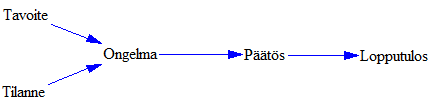
\includegraphics{tapahtuma}
\caption{Tapahtumasuuntautunut maailmankuva. \cite[s. 10]{Sterman2000} \label{sysdyn:tapahtumasuuntautunut}}
\end{figure}

Stermanin \cite[s. 11]{Sterman2000} mukaan sivuvaikutuksia ei ole todellisuudessa kuitenkaan olemassa. On vain olemassa vuorovaikutussuhteita, joita ei ole otettu huomioon. Seuraava kuva \ref{sysdyn:takaisinkytkentasuuntautunut} esittää takaisinkytkentäsuuntautunutta maailmankuvaa. Systeemiajattelijan maailmankuva on takaisinkytkentäsuuntautunut, ja hän ymmärtää päätösten vaikuttavan ympäristön tekijöihin, jotka puolestaan vaikuttavat päätöksiin. 

\begin{figure}[H]
\centering 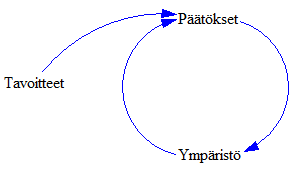
\includegraphics{takaisinkytkentasuuntautunut}
\caption{Takaisinkytkentäsuuntautunut maailmankuva. \cite[s. 11]{Sterman2000} \label{sysdyn:takaisinkytkentasuuntautunut}}
\end{figure}

Maailmankuvaa voi edelleen laajentaa. Seuraava kuva \ref{sysdyn:laajennettutakaisinkytkentasuuntautunut} on laajennettu edellisestä kuvasta \ref{sysdyn:takaisinkytkentasuuntautunut} ottamaan huomioon useampia systeemin tekijöitä. Systeemiajattelija hahmottaa, että päätöksillä on myös muita seurauksia, ja nekin muuttavat ympäristöä. Muuttuva ympäristö vaikuttaa myös tavoitteisiin -- niin omiin kuin muidenkin. Kun ympäristö ja muiden tavoitteet muuttuvat, tekevät muut päätöksiään sen pohjalta, mikä puolestaan muuttaa ympäristöä. \cite[s. 11--12]{Sterman2000}

\begin{figure}[H]
\centering 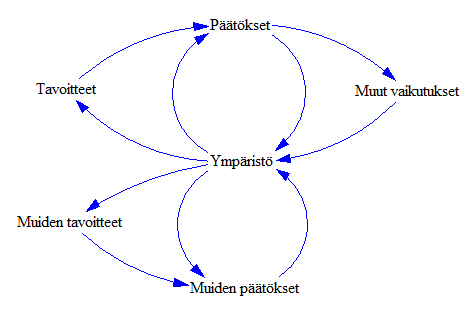
\includegraphics{laajennettutakaisinkytkentasuuntautunut}
\caption{Laajennettu takaisinkytkentäsuuntautunut maailmankuva. \cite[s. 11]{Sterman2000} \label{sysdyn:laajennettutakaisinkytkentasuuntautunut}}
\end{figure}


\subsection{Takaisinkytketyt systeemit \label{sysdyn:takaisinkytkenta}}

Systeemeissä on sisäsyntyisiä eli endogeenisiä (eng. endogenous) sekä ulkosyntyisiä eli eksogeenisiä (eng. exogenous) muuttujia. Sisäsyntyisen muuttujan arvo määräytyy systeemin sisäisen dynamiikan seurauksena, kun taas ulkosyntyisen muuttujan arvo annetaan systeemin ulkopuolelta, eikä näin ollen riipu systeemin tilasta. Ulkosyntyisisten muuttujien arvoista voidaan käyttää termiä "parametri". Parametrien arvot virittävät systeemin käyttäytymään tietyllä tavalla. \cite{Sterman2000} % Viiteviilausta

Systeemeillä on tuloja ja lähtöjä. Tulot (myös sisääntulo, eng. input) ovat systeemiin tulevia arvoja, jotka vaikuttavat systeemin käyttäytymiseen. Lähdöt (myös ulostulo, eng. output) ovat systeemin käyttäytymisestä seuraavia arvoja. Erilaisilla tuloilla saadaan systeemistä erilaiset lähdöt. Takaisinkytkentä (eng. feedback) tarkoittaa systeemin lähdön käyttämistä systeemin tulona. Tällöin systeemi kytkeytyy takaisin itseensä, muodostaa kytkennöistä silmukan (eng. loop) ja vaikuttaa itse itseensä. \cite{Sterman2000, WhatIsSystemDynamics} 

Stermanin \cite[s. 12]{Sterman2000} mukaan takaisinkytkennät vaikuttavat systeemin mutkikkuuteen enemmän kuin järjestelmän osien mutkikkuus itse. Tämän vuoksi takaisinkytkentöjen löytäminen on keskeisin osa systeemidynaamista mallinnusta. 

Systeemidynaamisia malleja esitetään kausaalidiagrammein, joihin merkitään systeemin osat eli muuttujanimet sekä niiden väliset vuorovaikutussuhteet kausaaliyhteysnuolten avulla. Nuolet piirretään lähtemään muuttujasta, joka vaikuttaa nuolen päätepisteen muuttujaan. Toisin sanoen nuoli kuvaa sitä, että nuolen alkupään muuttujan arvo eli lähtö toimii nuolen loppupään tulona. Nuoliin merkitään plus- tai miinusmerkki sen mukaan, kasvattaako vaiko vähentääkö lähtömuuttujan arvon kasvu tulomuuttujan arvoa. Nuolet piirretään kaareviksi, jotta systeemin dynamiikkaa, etenkin silmukat, olisi helpompi hahmottaa. \cite{Sterman2000}

Takaisinkytkettyjä silmukoita on kahdenlaisia: positiivisia ja negatiivisia. Positiiviset silmukat ovat itseään vahvistavia. Seuraavassa kuvassa \ref{sysdyn:positiivinen} on positiivinen takaisinkytketty silmukka, jossa kanojen määrä lisää munien määrää, mikä puolestaan lisää kanojen määrää. Positiiviset silmukat merkitään kausaalidiagrammiin kuvan \ref{sysdyn:positiivinen} mukaisesti R-kirjaimella, mikä tulee englannin kielen sanasta "reinforcing" eli suomeksi "vahvistava". \cite[s. 12--13]{Sterman2000}\cite{WhatIsSystemDynamics}

\begin{figure}[H]
\centering 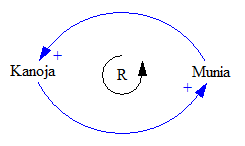
\includegraphics{positiivinen}
\caption{Positiivinen takaisinkytketty silmukka. \cite[s. 13]{Sterman2000} \label{sysdyn:positiivinen}}
\end{figure}

Negatiiviset silmukat ovat itseään tasapainottavia. Seuraavassa kuvassa \ref{sysdyn:negatiivinen} on negatiivinen takaisinkytketty silmukka, jossa kanojen lisääntyminen johtaa siihen, että useampi niistä ylittää tien ja jää auton alle, mikä puolestaan vähentää kanojen määrää, mikä puolestaan vähentää tien ylityksiä. Negatiiviset silmukat merkitään kuvan \ref{sysdyn:negatiivinen} mukaisesti B-kirjaimella, mikä tulee englannin kielen sanasta "balancing" eli suomeksi "tasapainottava". \cite[s. 12--14]{Sterman2000}

\begin{figure}[H]
\centering 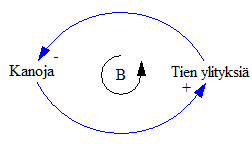
\includegraphics{negatiivinen}
\caption{Negatiivinen takaisinkytketty silmukka. \cite[s. 13]{Sterman2000} \label{sysdyn:negatiivinen}}
\end{figure}

Silmukka on positiivinen, kun siinä on parillinen määrä negatiivisia kytkentöjä. Kuvan \ref{sysdyn:positiivinen} positiivisessa silmukassa on nolla negatiivista kytkentää. Silmukka on negatiivinen, kun siinä on pariton määrä negatiivisia kytkentöjä. Kuvan \ref{sysdyn:negatiivinen} negatiivisessa silmukassa on yksi negatiivinen kytkentä. \cite[s. 12--14]{Sterman2000} Stermanin mukaan \cite{Sterman2011} viestittäessä takaisinkytkennöistä suurelle yleisölle, tulee välttää myönteisyyteen ja vastaisuuteen viittaavia termejä "positiivinen" ja "negatiivinen". Siksi tässä työssä käytetään silmukoiden yhteydessä termejä "vahvistava" ja "tasapainottava". 

\clearpage
\subsection{Viiveet, varastot ja virtaukset \label{sysdyn:vvv}}

Viiveet (eng. delay) aiheuttavat systeemiin hitautta, aiheuttavat värähtelyitä sekä johtavat siihen, että päätösten seuraukset johtavat pitkällä aikajänteellä erilaisiin tilanteisiin kuin lyhyellä aikajänteellä. Seuraavassa kuvassa \ref{sysdyn:viive} on esitetty systeemi, jossa hinnan nousu lisää viiveellä tuotantoa. Kausaalidiagrammeihin viiveet merkitään nuolen päälle joko kahdella poikkiviivalla tai laatikolla, jossa lukee "viive". \cite[s. 150--152]{Sterman2000} 

\begin{figure}[H]
\centering 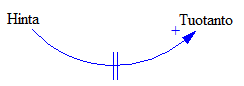
\includegraphics{viive}
\caption{Viiveellinen systeemi \cite[s. 150]{Sterman2000} \label{sysdyn:viive}}
\end{figure}

Varastot (eng. stock) ovat systeemin osia, joiden arvo kertyy. Ne tuottavat systeemiin muistia sekä hitautta ja niillä voi kuvata viiveitä. Varastot myös kertovat päättäjille, mikä on systeemin tila. Varastoon voi kohdistua virtauksia (eng. flow), jotka muuttavat varaston arvoa. Sisäänvirtaukset kerryttävät ja ulosvirtaukset kuluttavat varaston arvoa. Seuraava kuva \ref{sysdyn:varastovirtaus} on yksinkertainen kausaalidiagrammiesitys varastosta ja virtauksista. Varastot merkitään kausaalidiagrammiin suorakulmioilla, virtauskytkennät virtausnuolilla, virtausmuuttujat venttiilisymboleilla sekä systeemin ulkopuoliset lähteet (eng. source) ja nielut (eng. sink) pilvillä. \cite[s. 191--197]{Sterman2000} 

\begin{figure}[H]
\centering 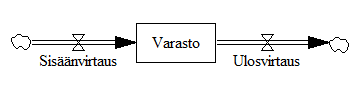
\includegraphics{varastovirtaus}
\caption{Yksinkertainen kausaalidiagrammi varastoista ja virtauksista. \cite[s. 150]{Sterman2000} \label{sysdyn:varastovirtaus}}
\end{figure}

Varaston matemaattinen esitys vastaa integraattoria, joka integroi sisäänvirtauksen ja ulosvirtauksen erotusta alkuhetkestä $t_0$ hetkeen $t$: 

\begin{equation}
  Varasto(t) = \int_{t_0}^t \Big( Sis\ddot{a}\ddot{a}nvirtaus(s) - Ulosvirtaus(s) \Big) ds + Varasto(t_0)
\end{equation} \cite[s. 194--195]{Sterman2000} 

Varastot ja virtaukset ovat intuitiivinen esitystapa, mutta saman dynamiikan voi esittää ilmankin niitä \cite[s. 191--230]{Sterman2000}. Seuraavassa kuvassa \ref{sysdyn:varastovirtauskana} on esitetty kuvan \ref{sysdyn:negatiivinen} negatiivisesti takaisinkytketty silmukka varastojen ja virtausten avulla. Kanojen määrä voidaan ajatella varastona ja tien ylitykset virtauksena, joka vähentää kanojen määrää. Kanojen määrä säätää tien ylitykset -venttiiliä: mitä enemmän kanoja, sitä avonaisempi venttiili ja suurempi virta. 

\begin{figure}[H]
\centering 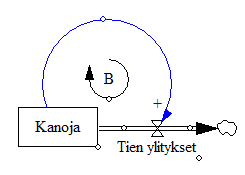
\includegraphics{varastovirtauskana}
\caption{Kuvan \ref{sysdyn:negatiivinen} negatiivisesti takaisinkytketyn silmukan esitys varastojen ja virtausten avulla. \label{sysdyn:varastovirtauskana}}
\end{figure}

Systeemidynamiikkaa käsittelevässä kirjallisuudessa käytetään usein kylpyammevertausta. Kylpyamme on varasto, jossa veden sisäänvirtaus tulee hanasta ja ulosvirtaus tapahtuu viemärin kautta. Jos sisäänvirtaus on suurempi kuin ulosvirtaus, kylpyammeen pinnankorkeus nousee ja päinvastoin, jos ulosvirtaus on suurempi, pinnankorkeus laskee. Kun virtaukset ovat yhtä suuret, systeemi on tasapainotilassa (eng. equilibrium). Vaikka konsepti on yksinkertainen, on ihmisillä vaikeuksia hahmottaa tällaista dynamiikkaa. Ihmiset kiinnittävät usein huomiota pelkästään sisään- tai ulosvirtaukseen sen sijaan, että kiinnittäisivät huomiota pinnankorkeuteen. Lopulta joudutaan tilanteeseen, jossa amme joko tulvii tai tyhjenee. \cite{Sweeney2000}

\section{Ilmastonmuutoksen mallintaminen \label{ilmasto}}

Ilmastonmuutos on tilastollisesti merkittävää ja pitkäkestoista muutosta globaalissa tai paikallisessa ilmastossa. Nykyisin tiedetään, että hiilidioksidi ja muut kasvihuonekaasut estävät maapallon lämpösäteilyä karkaamasta avaruuteen. Kasvihuonekaasujen lisääntyminen ilmakehässä aiheuttaa näin ollen ilmaston lämpenemistä. Tiedeyhteisössä vallitsee nykyisin konsensus, että ilmasto mitä todennäköisemmin lämpenee ihmisen toiminnan seurauksena, ja että se aiheuttaa merkittäviä haasteita ihmiskunnalle. Fossiilisten polttoaineiden käyttämisestä vapautuva hiilidioksidi on merkittävin tekijä, jolla ihminen aiheuttaa ilmastonmuutosta. \cite{AmericanInstituteofPhysics} 

Ilmastoa mallinnetaan ja simuloidaan, jotta ilmaston käyttäytymistä -- etenkin ilmaston lämpenemistä ja sen seurauksia -- ymmärrettäisiin paremmin. Kun ilmaston käyttäytyminen tunnetaan, voidaan tehdä valistuneita ilmastopoliittisia päätöksiä kasvihuonekaasupäästöjen leikkaamiseksi. \cite{CroadsFlightSimulator2011} Päästöjen leikkaaminen heikentää talouskasvua ja hyvinvointia lyhyellä aikajänteellä, mutta maksaa itsensä takaisin pitkällä aikajänteellä, kun ihmiskunnan ei tarvitse käyttää resurssejaan lämpenemisestä johtuvien ongelmien korjaamiseen. Kalliiksi tulee sekä liika päästöjen leikkaaminen että liian vähäinen päästöjen leikkaaminen. Leikkausten saavuttamiseksi voidaan käyttää monenlaisia keinoja päästöveroista päästöttömän energiatuotannon tukemiseen. Mallien avulla etsitäänkin optimaalisia leikkauksia sekä optimaalisia keinoja leikkausten saavuttamiseksi. \cite{Fiddaman2002}

Ilmastonmuutoksen mallintamiseen tarvitaan aina jonkinlainen fysikaalinen malli. Tarkimmissa fysikaalisissa malleissa ilmakehä ja meret saatetaan pilkkoa lukuisiin alueisiin ja useisiin kerroksiin. Näiden osien keskinäistä vuorovaikutusta simuloidaan erilaisin kasvihuonekaasujen määrin. Mitä tarkempi malli, sitä kauemmin sen simuloiminen kestää. \cite{CroadsFlightSimulator2011} 

Fysikaalista mallia voidaan laajentaa ottamalla huomioon ihmiskunnan ja ilmaston keskinäinen vuorovaikutus. Eri tieteenaloja yhdistelevistä malleista käytetään tässä työssä nimitystä yhdistetty malli (eng. integrated assessment model). Yhdistetyillä ilmastomalleilla voidaan esimerkiksi tutkia, miten ilmastonmuutos, väestönkasvu, talouskasvu ja hyvinvointi vaikuttavat toisiinsa. \cite{U.S.DepartmentofEnergy2009} 

Tässä työssä ilmastomalleja esiteltäessä ja vertailtaessa keskitytään systeemidynamiikan kannalta keskeisiin asioihin: Tutkitaan, mitä on mallinnettu ja jätetty mallintamatta, millaisia ovat mallin keskeiset takaisinkytkennät ja mitkä muuttujat on mallinnettu ulkosyntyisiksi. 

Tämän luvun tavoite on tutustuttaa lukija ilmastonmuutoksen mallintamiseen ensin yleisesti ja sitten systeemidynaamisiin malleihin pureutuen. Aluksi aliluvussa \ref{ilmasto:historia} otetaan katsaus ilmastotieteen, -mallien ja -politiikan historiaan. Historiaosuuden tavoite on auttaa ymmärtämään taustaa, miksi mallintamiseen on alettu käyttää myös systeemidynaamisia menetelmiä. Seuraavien alilukujen tavoite on esimerkkien kautta ymmärtää systeemidynaamisen ilmastomallinnuksen periaatteet. Aliluvussa \ref{ilmasto:croads} paneudutaan fysikaaliseen C-ROADS-ilmastomalliin. Tästä saavutettua ymmärrystä systeemidynaamisista ilmastomalleista laajennetaan aliluvuissa \ref{ilmasto:enroads} ja \ref{ilmasto:free} nopealla katsauksella yhdistettyihin systeemidynaamisiin En-ROADS- ja FREE-ilmastomalleihin.

\subsection{Ilmastotieteen, -mallien ja -politiikan historia \label{ilmasto:historia}}

Vuonna 1889 tiedemies Svante Arrhenius teki ensimmäiset laskelmat siitä, että hiilidioksidin lisääntyminen ilmakehässä aiheuttaisi ilmaston lämpenemistä. Hän kuitenkin arveli, että sen hetkisillä hiilidioksidipäästöillä ilmaston lämpeneminen useammalla asteella veisi tuhansia vuosia. Hän myös uskoi tämän olevan ihmiskunnan kannalta hyödyllistä. \cite{AmericanInstituteofPhysicsSimple}

1930-luvulla tehtiin ensimmäisiä havaintoja ilmaston lämpenemisestä. Keskustelu ilmaston lämpenemisestä jäi spekulaation tasolle, ja sitä pidettiin vain jonkinlaisena ilmastosyklinä. Lämpenemisen ei uskottu olevan ihmisen aiheuttamaa osittain siksi, että ihmistä pidettiin heikkona luonnonvoimien rinnalla. 1950-luvulla tehtiin ensimmäiset tieteelliset havainnot hiilidioksidin kertymisestä ilmakehään ja tästä seuraavasta ilmaston lämpenemisestä, mikä käynnisti ilmastonmuutoksen tutkimuksen. \cite{AmericanInstituteofPhysics} Vuonna 1950 kehitettiin ensimmäinen kaksiulotteinen ilmastomalli, jossa mallinnettiin Pohjois-Amerikan säätä 270:llä pisteellä, jotka olivat 700 km etäisyydellä toisistaan. Laskentatehoa ei tuolloin ollut vielä riittävästi, ja vuorokauden päähän tehdyn ennusteen laskeminen kesti vuorokauden. \cite{AmericanInstituteofPhysicsGCM}

Mallit ja laskentateho jatkoivat kehittymistä. Malleihin lisättiin erottelukykyä, ilmakehän kerroksia sekä maan pinnanmuotoja ja ne laajennettiin kattamaan koko maapallo. 1960-luvun puoliväliin tultaessa oli kehitetty ensimmäinen kaksikerroksinen koko maapallon kattava yleinen virtausmalli (eng. general circulation model), joka otti huomioon vuorten, merien ja jäätiköiden vaikutukset. \cite{AmericanInstituteofPhysicsGCM} Samaan aikaan tehtiin ensimmäiset löydökset ilmaston takaisinkytkennöistä, jotka saattaisivat tehdä ilmastosta yllättävänkin epävakaan. Ilmaston lämpenemistä ei kuitenkaan osattu nähdä vielä uhkana. \cite{AmericanInstituteofPhysics} 

Tarkkojen ilmastomallien lisäksi on kehitetty yksinkertaisia ilmastomalleja, joilla saatetaan esimerkiksi pureutua yksittäisiin ilmastokysymyksiin. Yksinkertaisissa malleissa maapallo voidaan esimerkiksi mallintaa yhtenä kokonaisuutena sen sijaan, että mallinnettaisiin ilmakehä lukuisiin palasiin jaettuna kolmiulotteisena hilana. Tällä tavalla ei tarvita niin paljoa laskentatehoa, mutta tutkittavan kysymyksen kannalta päästään riittävään tarkkuuteen. \cite{AmericanInstituteofPhysicsSimple} Seuraavissa aliluvuissa esiteltävät systeemidynaamiset mallit ovat yksinkertaisia ilmastomalleja, joista ensimmäisen julkaisi Tom Fiddaman väitöskirjassaan vuonna 1997 \cite{Fiddaman1997}. 

Ilmastotutkimus kehittyi hitaasti, mutta sai kunnon sykäyksen 1980-luvun loppulle tultaessa ilmastonmuutokseen jälleen havahduttaessa  \cite{AmericanInstituteofPhysics}. Tällöin perustettiin Hallitustenvälinen ilmastonmuutospaneeli IPCC (Intergovernmental Panel on Climate Change) kokoamaan ja arvioimaan ihmisen aiheuttaman ilmaston lämpenemistä ja sen vaikutuksia koskevaa tieteellistä tutkimusta. \cite{IPCChistory}. 

1990-luvulla ilmastomallit olivat päässeet ennusteissa jo hyvään tarkkuuteen \cite{AmericanInstituteofPhysics}. Tieteellinen tutkimus ei ole vieläkään antanut täyttä varmuutta kaikista ilmaston ominaisuuksista, joten ilmastomalleissa on väistämättä osia, jotka perustuvat spekulaatioon \cite{CroadsFlightSimulator2011}. Tästä syystä vuosikymmenten päähän ulottuvat ennusteet voivat antaa edelleen hyvin eriäviä tuloksia. Tästä huolimatta 2000-luvulle tultaessa tiedeyhteisö alkoi puhua jo konsensuksesta, että ilmasto mitä ilmeisimmin lämpenee ihmisen toiminnan seurauksena. Nyt tutkitaan, miten paljon ilmasto lämpenee, millaiset seuraukset sillä on ja miten sitä voitaisiin ehkäistä. \cite{AmericanInstituteofPhysics}

Ilmastonmuutoksen torjumiseksi perustettiin vuonna 1992 YK:n ilmastonmuutoskonventti UNFCCC (United Nations Framework Convention on Climate Change). Tämän työn kannalta keskeisimmät UNFCCC:n kokoukset ovat olleet Kioton, Cancúnin ja Kööpenhaminan ilmastokokoukset. Kioton ilmastokokouksessa vuonna 1997 lukuisat maat allekirjoittivat Kioton ilmastosopimuksen. Kioton ilmastosopimuksen ratifioineet maat sitoutuivat vähentämään tietyn prosenttiosuuden kasvihuonepäästöistään vuoden 1990 tasosta ilmastonmuutoksen hillitsemiseksi. Kioton sopimus sai seuraajakseen Kööpenhaminan sopimuksen vuonna 2009 ja vuonna 2010 Cancúnin sopimuksessa asetettiin tavoitteeksi, ettei maapallon keskilämpötila nousisi esiteollisesta ajasta yli 2\degree C:ta. \cite{UNFCCC} 

\subsection{C-ROADS-ilmastomalli \label{ilmasto:croads}}

Stermanin \cite{CroadsFlightSimulator2011} mukaan ilmastoneuvotteluissa on kaksi keskeistä haastetta liittyen ilmastomalleihin. Ensinnäkin päättäjien ja neuvottelijoiden on vaikea ymmärtää ilmastomalleja ja toisekseen tarkkojen ilmastomallien simuloimiseen erilaisilla skenaarioilla neuvotteluiden aikana ei ole aikaa. Neuvotteluissa eri maat asettavat eri oletusarvot esimerkiksi väestönkasvulle, joten on tärkeää, että simulaatiot kyetään ajamaan nopeasti paikan päällä eri kasvuodotusparametrein. Tämä sulkee pois tarkat ilmastomallit, ja Stermanin \cite{CroadsFlightSimulator2011} mukaan harva yksinkertaisistakaan ilmastomalleista on riittävän nopea. Malleja vaivaa myös se, että ne eivät ole välttämättä julkisesti ja helposti kaikkien saatavilla, ja niiden toimintaperiaatteita on vaikea ymmärtää. Ilman riittävää ymmärrystä ja sopivia työkaluja neuvottelijat ja päättäjät joutuvat siis turvautumaan omaan intuitioonsa. Tässä aliluvussa tutustutaan C-ROADS-ilmastomalliin ensin yleisesti sekä tutkitaan, miten mallilla on ratkaistu edellä mainittuja ongelmia. Tämän jälkeen tutustutaan mallin teknisen toteutuksen keskeisiin yksityiskohtiin. 

Climate Interactiven kehittämä C-ROADS (Climate-Rapid Overview And Decision Support) on yksinkertainen fysikaalinen ilmastomalli, joka perustuu Fiddamanin \cite{Fiddaman1997} kehittämään systeemidynaamiseen FREE-ilmastomalliin. C-ROADS:n keskeinen ulkosyntyinen muuttuja on kasvihuonekaasupäästöjen kehitys. Malliin voi asettaa myös haluamansa arvot esimerkiksi väestön ja bruttokansantuotteen kasvulle sekä herkkyysparametrille hiilidioksidin ilmastoa lämmittävälle vaikutukselle. \cite{CroadsFlightSimulator2011, Croads} C-ROADS on viritetty ja osoitettu toimivaksi historiadatan sekä tarkkojen fysikaalisten mallien avulla. Malli kykenee siis toistamaan historiadatan käyttäytymistä sekä antaa eri parametrein samoja ennusteita kuin parhaat tarkimmista ilmastomalleista  \cite{CroadsWWW, CroadsFlightSimulator2011}.

Mallia kehittäneen Stermanin mukaan \cite{Sterman2011} erinomainen tapa saada ihmiset ymmärtämään ilmastonmuutosta on interaktiivisten simulaatioiden avulla, jossa henkilö pääsee itse kokeilemaan erilaisten toimenpiteiden seurauksia. C-ROADS-malli on kehitetty tämän ajatuksen pohjalta. Mallin tarkoitus on auttaa ihmisiä ymmärtämään, miten ilmasto toimii ja millaiset pitkän aikajänteen seuraukset erilaisilla ilmastopoliittisilla päätöksillä kasvihuonekaasupäästöjen leikkaamiseksi on. \cite{CroadsWWW, CroadsFlightSimulator2011}

Mallista on pyritty kehittämään mahdollisimman nopea, läpinäkyvä ja helppokäyttöinen. C-ROADS-simulaation ajaa sekunnin murto-osassa, se on kattavasti dokumentoitu ja siinä on graafinen käyttöliittymä, jolla kuka tahansa voi kokeilla, millainen vaikutus erilaisilla kasvihuonekaasujen leikkauksilla ja kasvuodotusparametreilla on ilmastonmuutokseen. Graafisen käyttöliittymän avulla pääsee myös tarkastelemaan kausaalidiagrammeja, joista malli on rakennettu. C-ROADS-mallissa maapallon voi jakaa yhteen tai useampaan alueeseen, joista kukin tekee ilmastopoliittiset päätökset itsenäisesti. \cite{Croads, CroadsWWW, CroadsFlightSimulator2011} Kullekin valtiolle tai alueelle on määritetty omat bruttokansantuotteen ja väestönkasvun lukemat, jotka vaikuttavat syntyviin päästöihin \cite{Fiddaman2012}. Näin käyttäjä voi ajaa esimerkiksi simulaation tilanteessa, jossa Kiina vähentää päästöjään 50 \% alle vuoden 2000 tason ja muu maailma 40 \% alle vuoden 1990 tason. C-ROADS-mallin pohjalle on kehitetty myös roolipeli, World Climate, jossa kukin pelaaja edustaa eri maailman valtiota YK:n ilmastoneuvotteluissa. \cite{CroadsWWW} 

Climate Interactiven Andrew Jones \cite{Jones2013} kertoo, että he pitävät tyypillisesti kahden tunnin tilaisuuksia, joiden aikana osallistujat oppivat ymmärtämään C-ROADS:n avulla ilmaston dynamiikkaa ja ilmastopäätösten seurauksia. Osallistujat oppivat myös simuloimaan erilaisia skenaarioita C-ROADS:n avulla. 

C-ROADS onkin osoittautunut tehokkaaksi työkaluksi ja saanut laajaa suosiota. Lukuisat tutkijat, ympäristöministeriöt ja päättäjät ympäri maailman ovat ottaneet mallin käyttöönsä. \cite{CroadsWWW, CroadsFlightSimulator2011, Jones2013} 

C-ROADS-ilmastomallilla ennustettiin vuonna 2009, että ilmaston lämpenemisen rajoittamiseksi 2 \degree C:een olisi globaalisti hiilidioksidipäästöjä leikattava vuoteen 2050 mennessä 80 \% vuoden 1990 tasosta ja metsien tuhoutumisesta syntyviä päästöjä 90 \%  vuoden 2009 tasosta \cite{Sawin2009, Sterman2011}. Ennusteen tekijät kuitenkin huomauttavat C-ROADS jättää huomiotta osan mahdollisista ilmaston takaisinkytkennöistä tai antaa niille varovaisen takaisinkytkennän voimakkuutta määrittävän herkkyysparametrin. Tästä johtuen todellinen tarve kasvihuonepäästöjen vähennyksille saattaa olla ennusteen mukaista suurempi. \cite{Sawin2009, Sterman2011} Leikattavaa kasvihuonekaasupäästöissä olisi siis joka tapauksesa paljon enemmän, kuin millaisiin tavoitteisiin Kööpenhaminen ilmastokokouksessa päästiin vuonna 2009. \cite{UNFCCCCopenhagen, Sawin2009} 

C-ROADS:n arviointiryhmä antoi vuonna 2009 lausunnon, että malli ajaa asiansa: sen käyttäyttäytyminen noudattaa parhaiden ilmastomallien käyttäytymistä ja se toimii tehokkaana työkaluna kohdeyleisölle. Arviointiryhmä huomautti, että mallin pitäisi selkeämmin viestiä sen todellisia kykyjä mallintaa ilmastoa sekä kertoa epävarmuustekijöistä, jotka malliin liittyvät. Arviointiryhmä ehdotti myös, että malliin lisättäisiin osa pois jätetyistä takaisinkytkennöistä sekä Kioton ilmastosopimuksessa \cite{KyotoManual} mainittujen kasvihuonekaasujen rinnalle myös muut kasvihuonekaasut. \cite{Watson2009} Tässä työssä käytetään C-ROADS:n versiota 3.012.034 \cite{Croads}, johon on lisätty alunperin puuttuneita kasvihuonekaasuja ja takaisinkytkentöjä. 

C-ROADS-ilmastomalli koostuu useasta osamallista. Kullekin kasvihuonekaasulle on oma osamallinsa, samoin metsien kasvamiselle ja tuhoutumiselle, meren pinnan korkeudelle ja pH:lle sekä maapallolle kertyneelle lämpöenergialle. \cite{Croads, CroadsFlightSimulator2011, Fiddaman2012} Seuraavaksi tutustutaan C-ROADS:n teknisen toteutuksen kannalta keskeisiin lämpöenergian ja hiilidioksidin kiertokulkulkujen osamalleihin sekä mallin takaisinkytkentöihin. Havainnollistamisessa käytetään apuna mallin yksinkertaistettuja kausaalidiagrammeja. Diagrammeista on selkeyden vuoksi piilotettu vähemmän merkitykselliset muuttujat ja vuorovaikutukset sekä nostettu esille keskeiset yksityiskohdat. 

\subsubsection{Lämpöenergian kiertokulku \label{ilmasto:croads:lampo}}

Seuraava kuva \ref{ilmasto:lampo} on C-ROADS-ilmastomallin lämpöenergian kiertokulun kausaalidiagrammi. Mallissa on kaksi varastomuuttujaa lämpöenergialle: ilmakehä ja pintavedet sekä merten syvät kerrokset. Lämpöenergiaa systeemiin tulee vakionopeudella auringon säteilystä ilmakehään ja pintavesiin, josta se voi siirtyä joko merten syvyyksiin tai säteillä avaruuteen. \cite{Croads, CroadsFlightSimulator2011} 

\begin{figure}[ht]
\centering 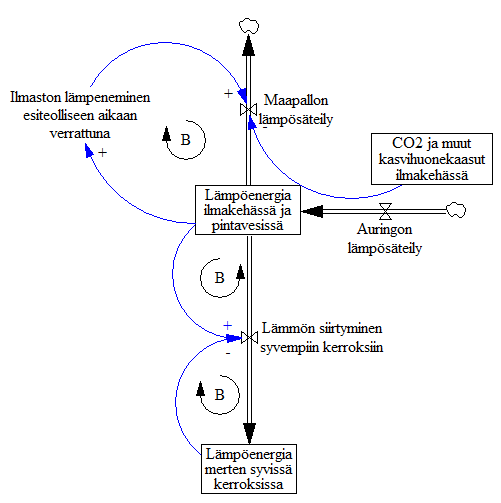
\includegraphics{c-roads-lampo}
\caption{C-ROADS-ilmastomallin lämpöenergian kiertokulku yksinkertaistettuna. \cite{Croads} \label{ilmasto:lampo}}
\end{figure}

Malliin on merkitty kolme tasapainottavaa silmukkaa. Alimmassa silmukassa merten syvien kerrosten lämpeneminen vähentää lämmön siirtymistä pintakerroksista syvempiin kerroksiin, mikä hidastaa syvien kerrosten lämpenemistä. Toisaalta keskimmäisessä silmukassa ilmaston lämpeneminen lisää lämmön siirtymistä syvempiin kerroksiin, mikä nopeuttaa syvien kerrosten lämpenemistä. Ylimmässä silmukassa ilmaston lämpeneminen lisää maapallon lämpösäteilyä avaruuteen, mikä vähentää ilmakehän ja pintavesien lämpöenergiaa. Hiilidioksidi ja muut kasvihuonekaasut puolestaan vähentävät maapallon lämpösäteilyä avaruuteen. Tällöin häiriintyy tasapaino, jossa ilmakehään tulee yhtä paljon lämpöenergiaa kuin sieltä lähtee. Kasvihuonekaasujen lisääntyessä ilmasto siis lämpenee, kunnes lämpöenergia alkaa jälleen virrata pois ilmakehästä yhtä nopeasti kuin sitä tulee auringon lämpösäteilystä. \cite{Croads, CroadsFlightSimulator2011} 

\subsubsection{Hiilidioksidin kiertokulku \label{ilmasto:croads:co2}}

Seuraava kuva \ref{ilmasto:co2} on yksinkertaistettu hiilidioksidin osamalli. Varastomuuttujat kuvaavat hiilidioksidia ilmakehässä ja biomassassa sekä merten pinta- ja syvissä kerroksissa. Hiilidioksidia tulee systeemiin ihmisen toiminnan seurauksena eli pääasiassa fossiilisten polttoaineiden käytöstä. Ihmisen toiminnan tuottama hiilidioksidi vapautuu ilmakehään. Ilmakehä vaihtaa hiilidioksidia biomassan ja merten pintakerrosten kanssa. \cite{Croads, CroadsFlightSimulator2011}

\begin{figure}[ht]
\centering 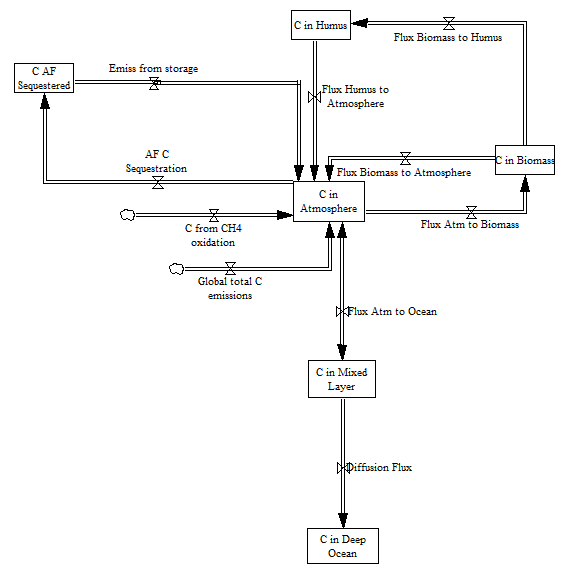
\includegraphics{c-roads-co2}
\caption{C-ROADS-ilmastomallin hiilidioksidin kiertokulku yksinkertaistettuna. \cite{Croads} \label{ilmasto:co2}}
\end{figure}

Ilmakehän hiilidioksidia liukenee merten pintakerroksiin, josta se voi liueta syvempiin kerroksiin. Virta ei ole kuitenkaan yksisuuntainen, vaan hiilidioksidi voi liueta syvemmistä kerroksista kohti pintaa ja vapautua pintakerroksista ilmakehään. Kuvaan \ref{ilmasto:co2} ei ole kausaaliyhteyttä sekavuuden välttämiseksi piirretty, mutta mitä enemmän ilmakehässä on hiilidioksidia ja mitä vähemmän sitä on merissä, sitä voimakkaammin sitä liukenee ilmakehästä meriin. Myös lämpötila vaikuttaa hiilidioksidin liukenemiseen mereen. Hiilidioksidi liukenee mereen sitä huonommin, mitä enemmän ilmasto lämpenee. \cite{Croads, CroadsFlightSimulator2011}

Biomassan kasvattaminen sitoo ilmakehän hiilidioksidia. Mallissa pystyy lisäämään biomassan määrää lisäämällä metsien kasvattamista sekä vähentämällä niiden tuhoutumista. Mallissa ainoat keinot vaikuttaa ilmakehän kasvihuonekaasujen määrään sekä siten ilmaston lämpenemiseen ovat päästöjen vähentäminen ja biomassan lisääminen. \cite{Croads}

Systeemiin tulee hiilidioksidia, mutta sitä ei poistu lainkaan. Systeemi muistuttaa siis tulpattua kylpyammetta, johon tulee koko ajan lisää vettä. Ammeen koko on periaatteessa rajaton, mutta hiilidioksidin virta biomassaan on rajallinen ja meriin ei mahdu loputtomasti hiilidioksidia. Jos hiilidioksidia ei enää pysty virtaamaan riittävästi meriin tai biomassaan, voi ilmakehän hiilidioksidipitoisuus ja siten ilmaston lämpeneminen lähteä räjähtävään kasvuun ilmankin, että päästöt lisääntyvät. Olennaista ei ole, kuinka paljon hiilidioksidia ilmakehään milläkin hetkellä vapautuu, vaan kuinka paljon sinne on aikojen saatossa hiilidioksidia vapautunut. Tämä on yksi keskeinen asia, jota ihmisten on vaikea hahmottaa. \cite{CroadsFlightSimulator2011} 

Todellisuudessa systeemistä poistuu jonkin verran hiilidioksidia -- tai tarkalleen ottaen hiiltä -- biomassan vapauttaessa metaania. Tämä on C-ROADS:ssa myös mallinnettu, mutta sen merkitys hiilidioksidin kiertokulun kannalta on pieni. \cite{Croads}

\subsubsection{Takaisinkytkennät \label{ilmasto:croads:takaisinkytkennät}}

Seuraava kuva \ref{ilmasto:co2-lampo} on esimerkki mallin takaisinkytkennästä, joka seuraa suoraan hiilidioksidin ja lämpöenergian kiertokulusta. Ilmakehässä olevan hiilidioksidin lisääntyessä heikentyy maapallon lämpösäteily avaruuteen, mikä hidastaa lämpöenergian poistumista ilmakehästä ja pintavesistä. Tämä johtaa ilmaston lämpenemiseen, mikä heikentää hiilidioksidin liukoisuutta meriin, mikä puolestaan lisää hiilidioksidin määrää ilmakehässä. \cite{Croads, CroadsFlightSimulator2011}

\begin{figure}[ht]
\centering 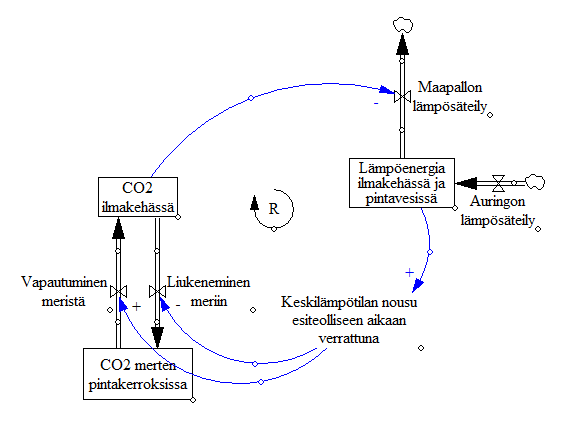
\includegraphics[width=\textwidth]{c-roads-co2-lampo}
\caption{C-ROADS-ilmastomallin mereen liuenneen hiilidioksidin ja ilmaston lämpenemisen vahvistava silmukka yksinkertaistettuna. \cite{Croads} \label{ilmasto:co2-lampo}}
\end{figure}

Mallissa on enemmänkin vastaavanlaisia takaisinkytkentöjä. Esimerkiksi biomassan kasvu tehostuu ilmakehän hiilidioksidin lisääntyessä ja toisaalta heikkenee ilmaston lämmetessä. Lisäksi ilmaston lämpeneminen lisää metaanin määrää ilmakehässä, sillä lämpeneminen vapauttaa metaania sulavasta ikiroudasta ja saa biomassan tuottamaan enemmän metaania. Metaani on kasvihuonekaasu, joten sen lisääntyminen ilmakehässä lämmittää ilmastoa. \cite{CroadsFlightSimulator2011}

Takaisinkytkentöjen voimakkuutta säädetään herkkyysparametrein. Osaan näistä takaisinkytkennöistä on laitettu varovaiset herkkyysparametrit tai ne on kytketty kokonaan pois päältä, sillä ilmastotiede ei ole vielä kyennyt osoittamaan takaisinkytkentöjen todellista voimakkuutta. \cite{CroadsFlightSimulator2011}

\subsection{En-ROADS-ilmastomalli \label{ilmasto:enroads}}

Climate Interactiven kehittämä En-ROADS (Energy-Rapid Overview And Decision Support) on FREE-ilmastomalliin pohjautuva, systeemidynaaminen, yhdistetty ilmastomalli. En-ROADS on laajennettu C-ROADS-ilmastomallista yhdistämällä malliin ihmiskunnan energiatuotanto ja talous. Siinä missä C-ROADS-malli keskittyi pääasiassa tutkimaan kasvihuonekaasupäästöjen leikkausten vaikutuksia ilmastoon, tutkii En-ROADS kokonaisvaltaisemmin energiatuotannon, talouden ja ilmaston keskinäisiä vaikutuksia. En-ROADS tutkii puhtaasti maailmanlaajuista kehitystä, eikä mallissa voi C-ROADS:n tavoin jakaa maailmaa itsenäisiin alueisiin. C-ROADS:n tavoin En-ROADS-simulaation ajaa sekunnin murto-osassa, vaikka se onkin paljon laajempi malli. \cite{EnroadsWWW, Harvey2013, Enroads} 

En-ROADS:n ulkosyntyiset muuttujat on jaettu oletuksiin ja olosuhteisiin sekä toimenpiteisiin ja päätöksiin. Ne on jaettu edelleen energiatuotannollisiin ja taloudellisiin muuttujiin. Oletusten ja olosuhteiden avulla käyttäjä voi syöttää malliin haluamansa uskomukset maailman kehityksestä ja kokeilla, millaisia tuloksia saadaan erilaisin toimenpitein ja päätöksin. Energiatuotanto on jaettu kahdeksaan eri muotoon: fossiilisiin kivihiileen, öljyyn ja maakaasuun, uusiutuviin bioenergiaan, vesivoimaan ja muihin uusiutuviin sekä ydinvoimaan ja uusiin energiatuotantomuotoihin. Eri tavat tuottaa energiaa vapauttavat ilmakehään eri määrän kasvihuonekaasuja. \cite{Enroads}

Mallissa voi tehdä useita erilaisia toimenpiteitä ja poliittisia päätöksiä energiatuotannon ja talouden ohjaamiseksi. Energiamuotoja voidaan verottaa tai tukea ja niiden houkuttelevuutta voidaan säätää, päästöille voidaan asettaa hinta, energiatehokkuutta voidaan parantaa ja uusien energiateknologioiden kehitykseen voidaan panostaa. Nämä toimenpiteet ja päätökset vaikuttavat energiatuotantoon ja talouteen sekä sen myötä päästöihin ja ilmaston lämpenemiseen. \cite{Harvey2013, Enroads} Harvey \cite{Harvey2013} esittää En-ROADS-ilmastomallilla tehtyjen tutkimusten perusteella, että lämpenemisen pysäyttäminen alle 2\degree C:een ei tarvitse tulla lyhyelläkään tähtäimellä erityisen kalliiksi, jos yhdistellään eri keinoja energiatehokkuudesta päästöveroihin. 

\subsection{FREE-ilmastomalli \label{ilmasto:free}}

FREE (Feedback-Rich Energy-Economy) on Tom Fiddamanin kehittämä systeemidynaaminen, yhdistetty ilmastomalli, jonka hän julkaisi väitöskirjassaan vuonna 1997. Malli on rakennettu Nordhausin DICE-ilmastomallin \cite{Nordhaus1992} pohjalta. \cite{Fiddaman1997} En-ROADS on hyvin pitkälti FREE:n pohjalta rakennettu malli, joten mallit ovat yleisellä tasolla hyvin samanlaiset. Fiddaman kritisoi \cite{Fiddaman2002}, että tyypillisesti sen aikaisissa yhdistetyissä malleissa on runsaasti ulkosyntyisiä muuttujia, äärettömiä ja lineaarisia hiilidioksidinieluja, sekä puutteelliset viiveet, takaisinkytkennät ja vuorovaikutukset. Lisäksi ne antavat enemmän painoarvoa rikkaiden maiden ja nykyisten sukupolvien hyvinvoinnille ja olettavat toimintaa täydellisen tiedon valossa. Näitä ongelmia Fiddeman on korjannut FREE-malliin. 

Seuraava kuva \ref{ilmasto:muut:free} on FREE-ilmastomallin rakenteen yleiskuva ylätason kausaalidiagrammilla kuvattuna. Malli koostuu yhdeksästä osamallista, joista kaksi on jätetty En-ROADS:ssa mallintamatta. Nämä osamallit ovat ihmiskunnan hyvinvointi sekä ilmastonmuutoksen aiheuttamat vahingot niin talouteen kuin ihmiskunnan hyvinvointiin. Ilmaston lämpeneminen heikentää kansantuotetta ja ihmisten hyvinvointia. Kansantuotteen kasvu puolestaan parantaa ihmisten hyvinvointia. \cite{Fiddaman1997, Fiddaman2002}

\begin{figure}[ht]
\centering 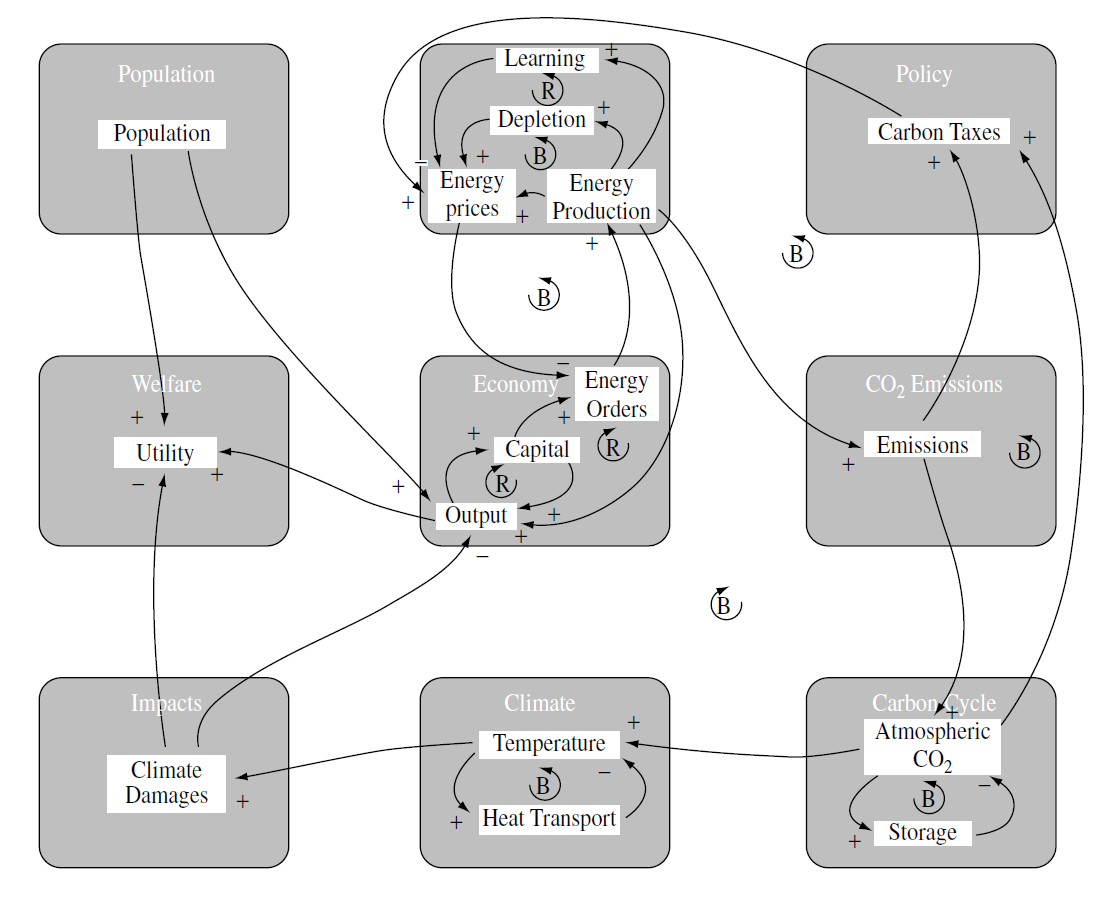
\includegraphics[width=\textwidth]{free}
\caption{FREE-ilmastomallin rakenne. \cite{Fiddaman2002} \label{ilmasto:muut:free}}
\end{figure}

Ilmaston lämpenemisen aiheuttamat vahingot lasketaan suoraviivaisesti ilmaston lämpenemisestä. Hyvinvoinnille on puolestaan kertymähyötyfunktio. Hyödyksi katsotaan ihmisten mahdollisuus kuluttaa, mikä syntyy kansantuotteesta. Kertymähyötyfunktio laskee tarkasteluajanjakson hyötykertymän. Kertymää voidaan painottaa hyvintasoeroja kuvaavalla parametrilla sekä sukupolvien välistä oikeudenmukaisuutta kuvaavalla parametrilla, jolla voidaan esimerkiksi asettaa nykyhetken hyödylle suurempi painoarvo kuin vuoden 2050 hyödylle. \cite{Fiddaman1997, Fiddaman2002} Fiddaman \cite{Fiddaman2002} on etsinyt mallin avulla optimaalista tapaa vähentää kasvihuonekaasupäästöjä ja osoittanut, että päästölupien sijaan päästöverot on parhaan hyvinvoinnin tuottava tapa vähentää kasvihuonekaasupäästöjä. 

\clearpage

\section{Yhteenveto ja pohdinta \label{yhteenveto}}

Tämän kandidaatintyön tavoitteeksi asetettiin tutkia systeemidynamiikan soveltamista ilmastonmuutoksen mallinnukseen ja simulointiin. Erityisesti oltiin kiinnostuneita tietämään, mitä lisäarvoa systeemidynamiikka tuo ilmastonmuutoksen mallintamiseen. Luvussa \ref{sysdyn} tutustuttiin työn kannalta välttämättömiin systeemidynamiikan perusperiaatteisiin: systeemiajatteluun, päätöksentekoon, takaisinkytkentöihin, viiveisiin, varastoihin ja virtauksiin. Luvussa \ref{ilmasto} otettiin katsaus ilmastotieteeseen ja ilmastonmuutoksen mallintamiseen sekä yleisesti että systeemidynamisiin malleihin syventyen. Aliluvussa \ref{ilmasto:croads} tutkittiin C-ROADS-ilmastomallia. Ensin tutustuttiin mallin ratkaisemiin ilmastoneuvotteluihin liittyviin ilmastomallien ongelmiin ja sitten mallin tekniseen toteutuksen keskeisiin osiin: lämpöenergian ja hiilidioksidin kiertokulkuihin sekä takaisinkytkentöihin. Tästä saavutettua ymmärrystä systeemidynaamisista ilmastomalleista laajennettiin aliluvuissa \ref{ilmasto:enroads} ja \ref{ilmasto:free} tutustumalla yhdistettyihin systeemidynaamisiin En-ROADS- ja FREE-ilmastomalleihin. Tässä luvussa käsitellään työssä tehtyjä löydöksiä. 

Systeemidynamiikassa keskitytään kausaalidiagrammien avulla tutkimaan takaisinkytkentöjä, epälineaarisuuksia, viiveitä, varastoja ja virtauksia. Tämä vaikuttaisi tehokkaalta lähestymistavalta yksinkertaisten ilmastomallien kehittämiseen, sillä systeemidynaamisten mallien ennusteet noudattavat historiadataa sekä parhaiden tarkkojen ilmastomallien ennusteita. Systeemidynaamisiin malleihin voidaan myös mallintaa spekulatiivisia osia, kuten takaisinkytkentöjä, joiden käyttäytymistä ei täysin tunneta. Niiden herkkyysparametreja säätämällä voidaan spekuloida systeemin todellista käyttäytymistä. Lisäksi systeemidynaamisen ilmastosimulaation ajaa sekunnin murto-osassa. Nämä ovat kuitenkin vain perusedellytykset hyvälle yksinkertaiselle ilmastomallille. 

Merkityksellisemmät hyödyt systeemidynamiikasta on mallin käyttäjälle, joka voidaan mallin avulla johdattaa oppivaksi systeemiajattelijaksi. Kausaalidiagrammien ilmaisuvoimaisuuden ansiosta systeemin vuorovaikutukset on kenen tahansa hahmotettavissa ainakin pääpiirteittäin. Kausaalidiagrammein voidaan ohjata tyypillisesti tapahtumaorientoituneesti ajatteleva käyttäjä hahmottamaan ilmaston takaisinkytkentöjä, epälineaarisuuksia, viiveitä, varastoja ja virtauksia. Sama ei onnistu matemaattisten yhtälöiden avulla. Myös mallin simulointi sekunnin murto-osassa helpottaa käyttäjää, joka voi hetkessä kokeilla, miten ilmasto muuttuu eri parametrien arvoilla. C-ROADS:n erityinen etu on mallin vapaa saatavuus ja malliin rakennettu käyttöliittymä, jotka tuovat ilmaston simuloinnin ja sen tutkimisen kenen tahansa saataville. 

On tyypillistä, että systeemidynaaminen malli tehdään jonkin ongelman ratkaisemisen tueksi, eikä niinkään mahdollisimman tarkkaa todellisuuden mallintamista varten \cite{Sterman2000}. Mitä ilmeisimmin tämän vuoksi Climate Interactivella on olemassa erikseen C-ROADS- ja En-ROADS-ilmastomallit, vaikka En-ROADS sisältääkin C-ROADS:n toiminnallisuuden. Samoin En-ROADS ei sisällä kaikkea FREE-mallin toiminnallisuutta, sillä mallit painottavat eri asioita. C-ROADS:lla tutkitaan päästöleikkausten vaikutuksia ilmaston lämpenemiseen ja En-ROADS:lla tutkitaan poliittisten päätösten ja toimenpiteiden vaikutuksia energiatuotantoon, talouteen, päästökehitykseen sekä siten ilmaston lämpenemiseen. FREE on puolestaan kuin En-ROADS, mutta tutkii asiaa vahvemmin ihmiskunnan hyvinvoinnin, hyvinvointierojen ja sukupolvien välisen oikeudenmukaisuuden näkökulmasta. 

Työssä keskityttiin jokseenkin yksipuolisesti Climate Interactiven sekä siinä mukana olevien Stermanin ja Fiddamanin tutkimuksiin ja systeemidynaamisiin ilmastomalleihin. Tämä johtuu siitä, että muita systeemidynaamisia malleja löytyi vain yksi \cite{Evan2007}, ja sekin pohjautuu FREE-ilmastomalliin. Muut löydetyt systeemidynaamiset ilmastonmuutosta läheisesti käsittelevät mallit keskittyivät pääasiassa tutkimaan energiatuotantoa ja päästöjä \cite{Kunsch2003, Shrestha2012, Mediavilla2013}. Systeemidynamiikka on kuitenkin vain eräänlainen esitystapa ja ajatusmalli. Fiddaman oli ilmastonmuutoksen systeemidynaamista mallinnusta tutkiessaan ja FREE-ilmastomallia kehittäessään tehnyt DICE-ilmastomallista systeemidynaamisen esityksen. Sama onnistunee myös muille yksinkertaisille ilmastomalleille. Kuten mainittua, systeemidynaamisten mallien etu ei niinkään kumpua matemaattisista yhtälöistä, vaan kausaalidiagrammien ilmaisuvoimasta sekä pyrkimyksestä ohjata ihmiset systeemiajatteluun. 

Tälle työlle jatkotutkimuksena voisi systeemidynaamisten ja muiden mallien ilmaisuvoimaa vertailla keskenään. Lisäksi, Fiddamanin tavoin, voisi muita yksinkertaisia ilmastomalleja tutkia systeemidynamiikan perspektiivistä. 

Näkisin, että systeemidynamiikka soveltuu erinomaisesti yksinkertaisten fysikaalisten ja yhdistettyjen ilmastomallien kehittämiseen. Systeemidynamiikka ja -ajattelu parhaimmillaan helpottavat todellisuutta vastaavan mallin luomista. Niiden suurin etu syntyy kuitenkin systeemidynaamisista kausaalidiagrammeista, joiden ilmaisuvoimalla voi johdattaa ihmiset ymmärtämään systeemin dynamiikkaa. 

%Julkista kritiikkiä tässä työssä esitettyjä malleja kohtaan ei C-ROADS-mallin arviointiryhmän raportin \cite{Watson2009} lisäksi löytynyt. Kritiikin puute voi selittyä useasta asiasta. C-ROADS ja En-ROADS ovat varsin uusia ja jatkuvan kehityksen alaisia malleja, eikä niistä ole juurikaan tehty julkaisuja. Tämä ei ole omiaan kerryttämään kritiikkiä niitä kohtaan. Systeemidynamiikassa on tyypillistä keskittyä osoittamaan malli vääräksi \cite{Sterman2000}, joten mallit ovat olleet jatkuvassa kriittisessä tarkastelussa, ja pahimmat ongelmat ovat mitä todennäköisemmin hioutuneet pois jo kehitysvaiheessa. Asiaa voi selittää myös systeemidynaamisen mallinnuksen omalaatuisuus, jota voi olla vaikea lähteä kritisoimaan, ellei ole systeemidynamiikan asiantuntija. Toisaalta ne systeemidynamiikan asiantuntijat, jotka ovat enemmän tekemisissä ilmastonmuutoksen kanssa, ovat luultavimmin mukana Climate Interactivessa. % Onko tämä nyt järkevää settiä? 



\clearpage
\phantomsection
\addcontentsline{toc}{section}{Viitteet}
%\bibliography{viitteet}
%\bibliographystyle{plain}
\printbibliography
%\pagestyle{plain}

\end{onehalfspacing} % KYPSYYSNÄYTETTÄ VARTEN


\end{document}

